\documentclass[11pt,oneside,a4paper]{article}
%define the title
\usepackage{graphicx}
\usepackage{listings}
\usepackage{setspace}
\usepackage{float}
\usepackage{titlesec}
%\usepackage{indent}
%\usepackage[labelfont=bf, textfont=normalfont, singlelinecheck=off, justification=raggedright]{caption}
% \titleformat*{\section}{\Large}
% \titleformat*{\subsection}{large}
% \titleformat*{\subsubsection}{normalsize}
\author{Group}
\title{Final_Report}
\begin{document}
\begin{titlepage}
\begin{center}
{\large \textsc{COMP2043.GRP Interim Group Report}}

\vspace{0.025\textheight} % Whitespace between the title and short horizonta
{\huge \textsc{Sequential Monte Carlo}} % Author name

\vspace{0.045\textheight}
{\huge\textsc{Team 6}}
\vspace{0.05\textheight}

{\huge\textsc{ 2017.12.7}}
\vspace{0.45\textheight}


\textbf{Supervisor:} Dr. Liang Dai
\vspace{0.045\textheight}

\textbf{Member:}
\begin{spacing}{2.0}%%�м�����Ϊdouble-space
          Hejia Qiu zy18720

          Cong Liu zy19426

          Zexi Song zy15777

          Xiang Zhang zy18743

          Kaiwen Zhang zy18672
\end{spacing}
  	\vspace{0.025\textheight}
\end{center}
\end{titlepage}
\tableofcontents
\newpage
\section{Introduction}

\subsection{Background of the Project}
Sequential Monte Carlo(SMC, also called particle filter), is a widely-used statistical sampling method, which is
used to sequentially sample from a sequence of target densities. It deals with the problem of recursively estimating
the probability density function $ p(x_t|Y_s) $.
\newline Befort the short journey of Introduction to Particle filter, a brief Background of particle filter will be explained firstly. In our present world, the ability
of solve the problem of estimating various quantities in nonlinear dynamic systems is of paramount importance in many
practical applications. In order to understand how a system, for instance, a aircraft, a car, or a camera performs, we
need to have access to certain important quantities related with the system. However, typically we have to estimate them
based on various noisy measuremets available from the sytem due to the fact that we do not have direct access to these factors.
According to Thomas B.Schon, the state estimation problem is addressed mianly within a probabilistic framework. More specifically,
the approach is heavily affected by the Bayesian view of estimation, which implies that the complete solution to the
estimation problem is provided by the probability density function $ p(x_t|Y_s) $. This density function contains all available
information about the state variable.

\subsection{Motivation \& Wide implmentation of state estimation}
The automotive industry's focus is recently shifting from mechanics to electronics and software. This opens up factors
a great deal of interesting applications and research opportunities within the field of estimation theory.
\begin{figure}[H]
  \begin{center}
  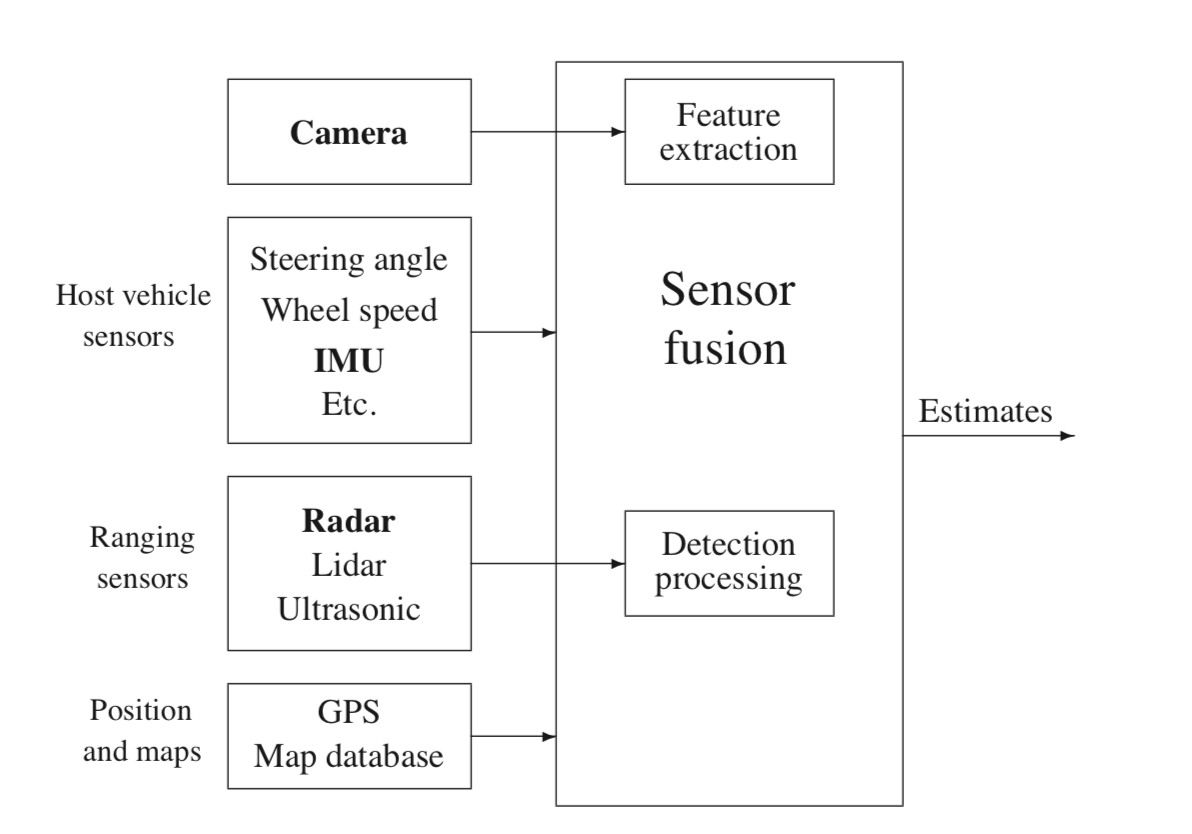
\includegraphics[height=0.3\textheight]{./source/1.png}
  \end{center}
  \caption{ The most important factors enabling future automative safety systems
  is the availablility of accurate information about the state. The process of obtaining
  this information is to a large extent dependent on a unified treament of the sensor information, as illustrated
  in this figure.}
  \label{}
\end{figure}
\subsubsection{Automotive Navigation-Example}
The objective of this study is to calculate estimates of the road geometry,
which are important in several advanced control systems such as lane guidance
and collision avoidance.

\begin{figure}[H]
  \begin{center}
  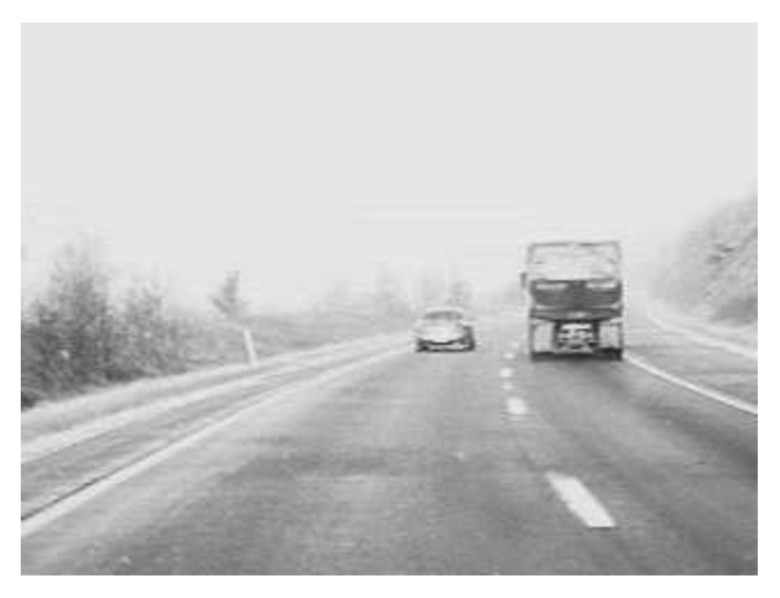
\includegraphics[height=0.3\textheight]{./source/2.png}
  \caption{when entering a curve, all vehicles start moving in the lateral direction. This information
  can be used to support the road geometry estimate.}
  \label{}
  \end{center}
\end{figure}

Assuming that the surrounding vehicles will keep following the same lane, is in discrete-time expressed as
$y{_t+1}^i = y_{t}^i + w_t,\qquad w_t \sim \mathcal{N}(0, \mathcal{Q}_{lat}). $ Here, $y^i $ denotes the lateral
position of vehicle $i $ and $w_t $ denotes Gaussian white noise which is used to accout for model uncertainties.
The estimate of the road curvature during an exit phase of a curve is illustrated in Figure 3. The true reference
signal was generated using the method proposed by Eidehall and Gustafsson (2006).

\begin{figure}[H]
  \begin{center}
  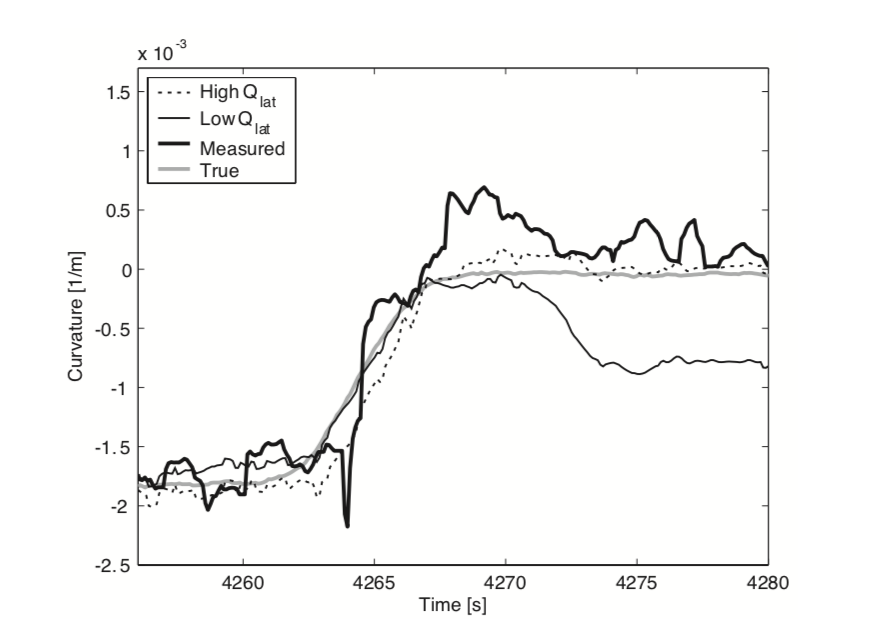
\includegraphics[height=0.3\textheight]{./source/3.png}
  \caption{Comparision of estimation performance from two filters, one with a large $\mathcal{Q}_{lat} $ and one with a small $\mathcal{Q}_{lat} $. The raw measuremet signal from the image processing
  unit is also included. Comparing this raw vision measuremet to the result from the filters clearly illustrates the power of a model based sensor fusion approach}
  \label{}
  \end{center}
\end{figure}

\subsubsection{Navigation for Augmented Reality}
\begin{figure}[H]
  \begin{center}
  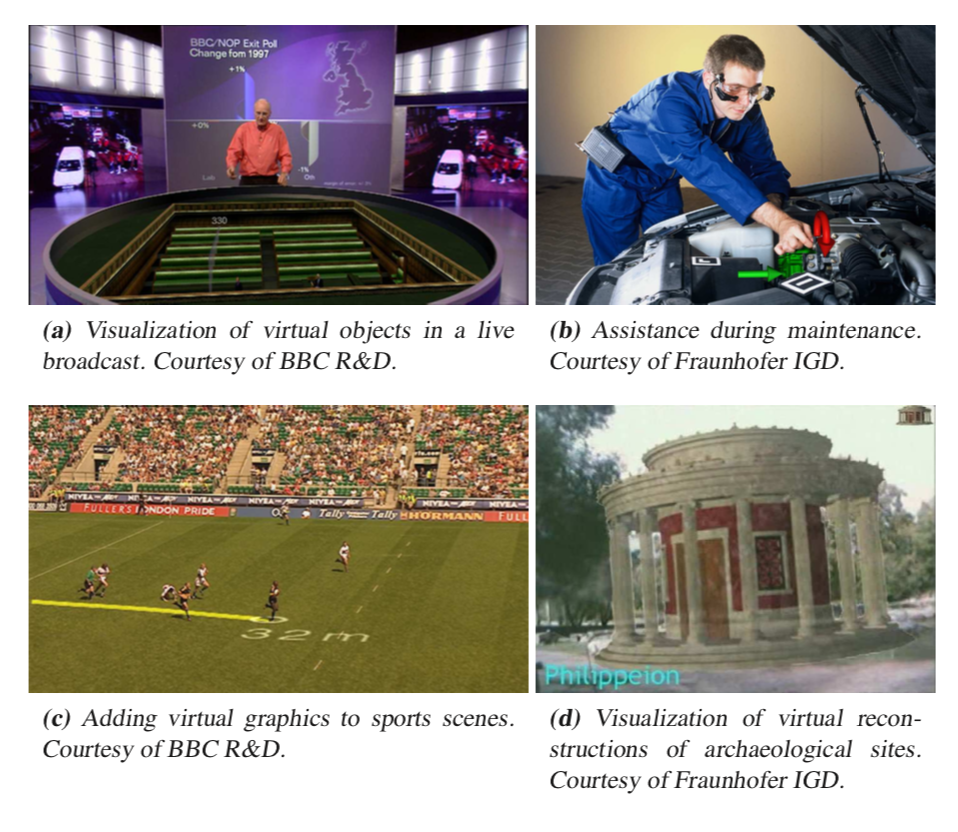
\includegraphics[height=0.2\textheight]{./source/4.png}
  \caption{Some examples illustrating the concept of augmented reality.}
  \label{}
  \end{center}
\end{figure}

\subsection{Scope of the project}
This subsection describes the scenario where the product will be used for.

\subsection{Introducing two auxiliary particle filters(APF)}
\subsubsection{Bootstrap particle filter}

\subsubsection{Fully adapted particle filter}























\end{document}
